% Independently authored compatible ReScience layout.
% ReScience/template style reference: 0978d0e5d9a86246789fd3468aec6fc71e39c944.
\documentclass[a4paper,10pt]{article}
\usepackage[a4paper,left=4.5cm,right=3cm,top=3cm,bottom=3.5cm,headheight=14pt,footskip=1.5cm]{geometry}
\usepackage{fontspec}
\defaultfontfeatures{Ligatures=TeX}
\setmainfont{SourceSerifPro-Light.otf}[Path=fonts/,ItalicFont=SourceSerifPro-LightIt.otf,BoldFont=SourceSerifPro-Regular.otf,BoldItalicFont=SourceSerifPro-It.otf]
\setsansfont{RobotoCondensed-Light.ttf}[Path=fonts/,BoldFont=RobotoCondensed-Regular.ttf,ItalicFont=RobotoCondensed-LightItalic.ttf]
\setmonofont{SourceCodePro-Light.otf}[Path=fonts/,BoldFont=SourceCodePro-Regular.otf]
\usepackage{graphicx,xcolor,longtable,array,booktabs,titlesec,fancyhdr,amsmath}
\usepackage[unicode,hidelinks,breaklinks]{hyperref}
\usepackage{xurl}
\urlstyle{same}
\definecolor{draftred}{HTML}{A72A34}
\titleformat{\section}{\Large\sffamily\bfseries}{}{0pt}{}
\titleformat{\subsection}{\large\sffamily\bfseries}{}{0pt}{}
\titlespacing*{\section}{0pt}{15pt}{7pt}
\titlespacing*{\subsection}{0pt}{12pt}{5pt}
\setlength{\parindent}{0pt}
\setlength{\parskip}{6pt plus 1pt}
\setlength{\tabcolsep}{3pt}
\renewcommand{\arraystretch}{1.18}
\pagestyle{fancy}\fancyhf{}
\fancyhead[L]{\scriptsize\sffamily Replication manuscript}
\fancyhead[R]{}
\fancyfoot[L]{\scriptsize\sffamily Byungwoong Yoo}
\fancyfoot[R]{\scriptsize\sffamily\thepage}
\renewcommand{\headrulewidth}{0pt}
\emergencystretch=2em
\hypersetup{pdfauthor={Byungwoong Yoo},pdfsubject={Replication manuscript},pdfkeywords={replication,transcriptomics,Python}}
\hypersetup{pdftitle={[¬Re] Halofantrine protects photoreceptors in multiple models of retinal degeneration: transcriptomic analyses}}
\begin{document}
{\sffamily\small Replication manuscript\par}
\vspace{6pt}

{\LARGE\sffamily\bfseries\raggedright\hyphenpenalty=10000 [¬Re] Halofantrine protects photoreceptors in multiple models of retinal degeneration: transcriptomic analyses\par}
\vspace{8pt}
{\sffamily\bfseries Byungwoong Yoo\par}
{\small\sffamily Independent Researcher\par}
{\small\sffamily ORCID: \href{https://orcid.org/0009-0002-1797-3100}{0009-0002-1797-3100}\par}
{\small\sffamily\href{mailto:yoonge3@gmail.com}{yoonge3@gmail.com}\par}
\vspace{8pt}
{\small\sffamily Code: \url{https://github.com/ByungwoongYoo/e071-halofantrine-reanalysis/tree/4a1b699d46e0895ab99d980faa61c45dc20c61f2}\par}
\section*{Abstract}
Kim et al. reported halofantrine-associated photoreceptor protection in three inherited retinal degeneration models and partial similarity in their transcriptomic responses. We examined the computational evidence accompanying that result, using the deposited differential-expression tables and normalized expression matrices for human CEP290-LCA retinal organoids, P23H rats and rd10 mice. Nine reconstructions of the gene-selection and mapping procedure did not reproduce the seven regions of Figure S7A and its sole three-model intersection. The deposited rd10 Itpr3 result had nominal p = 0.119, leaving unresolved which test supports the source statement of significance in all three models. These are gaps in recovering the specified analyses, not evidence that no valid implementation exists. Separately, multiple-testing control, one-to-one orthologue comparisons, leave-one-out analyses, overlap randomization and ranked pathway enrichment characterized the sensitivity of the transcriptomic interpretation. Human–rd10 effect concordance remained positive across all tested single-sample deletions; correlations involving P23H were weaker and crossed zero. Oxidative phosphorylation had positive enrichment scores in all three models, although only P23H met the chosen FDR threshold. The reanalysis identifies the source details needed to reproduce the two transcriptomic figures and provides quantitative robustness results without reassessing the reported phenotypic rescue.

\section*{1. Scope of the replication}
The source is the first version of \emph{Halofantrine protects photoreceptors in multiple models of retinal degeneration}, posted on Research Square on 13 May 2026 [1]. It reports experiments in human CEP290-LCA retinal organoids, P23H rats and rd10 mice, including photoreceptor protection and transcriptomic analyses. The source already acknowledges partial molecular similarity. Our target is the transcriptomic component, particularly Supplementary Figure S7A, the ITPR3/Itpr3 comparison in S7B, and the deposited expression results. We did not reanalyse the histological or functional experiments and do not treat the preprint as a peer-reviewed publication.

The public record allows some questions to be answered directly. It provides per-gene effect estimates, statistical tests and normalized expression matrices. Other results require choices not uniquely specified by those files: the ordering of filtering and ranking, conversion to human gene identifiers, the particular samples and test used for a plotted comparison, and the biological meaning of sample prefixes. We distinguish attempts to recover those source analyses from additional analyses whose methods we chose ourselves.

{\small
\begin{longtable}{>{\raggedright\arraybackslash}p{\dimexpr 0.22\linewidth-2\tabcolsep\relax}>{\raggedright\arraybackslash}p{\dimexpr 0.29\linewidth-2\tabcolsep\relax}>{\raggedright\arraybackslash}p{\dimexpr 0.49\linewidth-2\tabcolsep\relax}}
\toprule
\textbf{Target} & \textbf{Evidence examined} & \textbf{Result of this replication} \\
\midrule
\endfirsthead
\toprule
\textbf{Target} & \textbf{Evidence examined} & \textbf{Result of this replication} \\
\midrule
\endhead
\bottomrule\endfoot
Deposited HAL-versus-DMSO effect estimates & Differential-expression tables and normalized CPM matrices & Mean differences in transformed CPM closely track the deposited log-fold changes; the source differential-expression model was not refitted. \\
Figure S7A gene overlap & Source diagram, methods and nine explicit selection/mapping reconstructions & No tested rule recovers both the region counts and sole all-three ITPR3 intersection. The exact source implementation remains unresolved. \\
Figure S7B and the all-three significance statement & Deposited ITPR3/Itpr3 rows, CPM values and figure labels & The rd10 deposited test is not nominally significant. The source figure's test and sample inclusion have not been recovered. \\
Human-organoid replication structure & GEO sample names and metadata & HAL samples use PA/PB and DMSO samples PC/PD. What those prefixes encode remains unresolved. \\
Sensitivity of cross-model comparisons & Explicit additional analyses of the same deposited data & Quantified with multiple-testing thresholds, effect correlations, deletion tests, list-size-preserving nulls and ranked GSEA. These are not exact replications of the source pathway procedure. \\
\end{longtable}
}
\section*{2. Data and implementation}
\subsection*{2.1 Deposited data and experimental units}
The three series are GSE327431 (human CEP290-LCA), GSE327432 (P23H rat) and GSE327434 (rd10 mouse), under SuperSeries GSE327435 [2]. For each, we used the deposited differential-expression CSV and normalized gene-level counts-per-million (CPM) matrix. The HAL/DMSO groups contained 5/5 human-organoid samples, 4/5 P23H samples and 3/3 rd10 samples. The ten human samples are labelled with the same patient donor, PEN1B; they are not ten independent patients. Their precise culture and technical replicate structure is not established by the metadata inspected here.

Input checks verified unique unversioned Ensembl identifiers, finite numerical values, p-values within [0,1], non-negative CPM, matching identifiers between expression and differential-expression files, and disjoint treatment groups with the expected sizes. Wild-type or familial-control columns were excluded from the treatment comparisons. Source accession URLs and compressed-file hashes identify the six expression inputs.

The source describes Kallisto, tximport, edgeR and limma with Ensembl release 115. It also cites an earlier retinal-analysis pipeline [3]. We reused the deposited logFC, moderated t-statistic, P.Value and adj.P.Val columns rather than claiming to repeat raw-read processing or refit that model. Counting genes under a new threshold is therefore an analysis of the source's estimates, not an independently fitted differential-expression result.

\subsection*{2.2 Identifier mapping and source-figure reconstruction}
Two mapping tasks were kept separate. For effect comparisons and robustness analyses we used frozen Ensembl BioMart one-to-one human–mouse–rat mappings [4]. The core snapshot contains 15,956 mappings; the symbol-bearing snapshot used for GSEA contains 15,940. They were preserved on 21 September 2026. The historical runs had queried the live service without retaining hashes, so equal row counts and reproduced results cannot establish byte-for-byte identity with those earlier inputs.

Recovering S7A is a different task: its legend describes conversion to human aliases, not necessarily our one-to-one restriction. In the nine reconstructions reported below, animal genes were mapped through all returned human homologues without a one-to-one filter; the selected human list was not restricted to the three-species universe. Nine rules combined nominal p-value and fold-change filters with ranking by absolute logFC, nominal p-value or absolute moderated t-statistic, top-500 selection, and balanced up/down selection. The code, inputs, mapped-list sizes, three-way intersection identifiers and seven Venn-region counts are preserved. We measured discrepancy by the sum of absolute differences between reconstructed and source region counts. This is a finite comparison of specified rules, not a search over every possible implementation.

\subsection*{2.3 Effect estimates and sample-deletion analyses}
For gene-level summaries, we applied either nominal p < 0.05 or deposited adjusted p < 0.05, together with |logFC| \ensuremath{\geq} log2(1.2). Pairwise cross-model comparisons used one-to-one orthologues represented in both datasets and reported Pearson and Spearman correlations, cosine similarity and sign concordance. Pairwise gene counts can exceed the intersection represented in all three datasets.

From each CPM matrix we computed the difference between HAL and DMSO means after transforming each value as log2(CPM + 0.5). This transformation supplies a transparent descriptive contrast; it does not reproduce all weighting, variance moderation or design terms of the source model. Each of the 25 disease samples was then omitted once. Within-model comparisons measured stability relative to the full effect vector, and all 257 full/deletion-state pairings were compared across model pairs. The resulting ranges are sensitivity ranges, not confidence intervals or independent replications.

For a separate global separation diagnostic, genes with nonzero finite variance were z-scaled across disease samples. The mean squared difference between treatment-group centroids was evaluated across every label assignment preserving group sizes: 252, 126 and 20 assignments. The reported tail fractions use the specified sample-label exchangeability assumption. In particular, unresolved culture or batch structure can invalidate a causal interpretation of the human diagnostic.

\subsection*{2.4 Overlap and pathway extensions}
The overlap extension first applied nominal p < 0.05 and the 1.2-fold-change gate, then selected up to 500 upregulated and 500 downregulated genes within each model. This is a documented interpretation of the source-like selection language, not the recovered S7A recipe. Mapped lists were restricted to the common 8,645-gene one-to-one universe. We compared genes appearing in at least two lists, and in all three, with 10,000 uniformly sampled sets preserving the three list sizes. Monte Carlo tail probabilities used the plus-one correction. This null conditions on list size but does not preserve co-expression, gene-specific detectability or pathway structure.

For the pathway extension, genes were ranked by the deposited moderated t-statistic, with symbol-based tie ordering, and restricted to a common 8,644-symbol universe. GSEApy prerank [5] tested KEGG\_2021\_Human [6,7] sets containing 10–500 represented genes, with 2,000 permutations and seed 20260921. There were 277 eligible pathways per model. This ranked analysis differs from the source's gProfiler-based mapping of selected DEGs; disagreement is not an exact failure to reproduce that procedure. We report the returned enrichment scores and FDR estimates at a reporting threshold of 0.05. A returned zero FDR is a finite-permutation estimate, not a literal probability of zero.

\section*{3. Recovery of the source transcriptomic results}
\subsection*{3.1 The tested S7A rules leave a specific reconstruction gap}
The source diagram corresponds to 500 human genes, 412 P23H human-mapped genes and 435 rd10 human-mapped genes, with ITPR3 alone in the intersection of all three. None of the nine tested rules recovered both this intersection and the seven region counts. The smallest summed absolute region-count difference was 72.

The closest tested reconstruction used nominal p < 0.05 followed by ranking on absolute logFC and top-500 selection. It excluded rd10 Itpr3 because its deposited p-value was 0.119. Removing the p-value filter admitted ITPR3 to all three top-|logFC| lists, but produced eight all-three genes rather than one. These alternatives show how the filtering and ranking choices affect the intersection. They do not identify which procedure the source authors used, and the failing candidates do not prove that the displayed figure is erroneous.

{\small
\begin{longtable}{>{\raggedright\arraybackslash}p{\dimexpr 0.1\linewidth-2\tabcolsep\relax}>{\raggedright\arraybackslash}p{\dimexpr 0.31\linewidth-2\tabcolsep\relax}>{\raggedright\arraybackslash}p{\dimexpr 0.18\linewidth-2\tabcolsep\relax}>{\raggedright\arraybackslash}p{\dimexpr 0.1\linewidth-2\tabcolsep\relax}>{\raggedright\arraybackslash}p{\dimexpr 0.13\linewidth-2\tabcolsep\relax}>{\raggedright\arraybackslash}p{\dimexpr 0.18\linewidth-2\tabcolsep\relax}}
\toprule
\textbf{Rule} & \textbf{Selection before human-homologue mapping} & \textbf{Mapped list sizes, H/R/M} & \textbf{All-three genes} & \textbf{ITPR3 in all three?} & \textbf{Summed region-count difference} \\
\midrule
\endfirsthead
\toprule
\textbf{Rule} & \textbf{Selection before human-homologue mapping} & \textbf{Mapped list sizes, H/R/M} & \textbf{All-three genes} & \textbf{ITPR3 in all three?} & \textbf{Summed region-count difference} \\
\midrule
\endhead
\bottomrule\endfoot
Source S7A & Source diagram; exact selection procedure unresolved & 500 / 412 / 435 & 1 & Yes & 0 \\
R1 & Top 500 by absolute logFC & 500 / 438 / 397 & 8 & Yes & 139 \\
R2 & Lowest 500 nominal p-values & 500 / 464 / 475 & 0 & No & 104 \\
R3 & Top 500 by absolute moderated t-statistic & 500 / 464 / 475 & 0 & No & 104 \\
R4 & Fold-change gate, then top 500 by absolute logFC & 500 / 438 / 397 & 8 & Yes & 139 \\
R5 & Nominal p-value gate, then top 500 by absolute logFC & 500 / 446 / 408 & 0 & No & 72 \\
R6 & Both gates, then top 500 by absolute logFC & 500 / 446 / 213 & 0 & No & 266 \\
R7 & Top 250 upregulated and 250 downregulated genes & 500 / 439 / 387 & 9 & Yes & 164 \\
R8 & Nominal p-value gate, then top 250 in each direction & 500 / 451 / 379 & 0 & No & 104 \\
R9 & Both gates, then top 250 in each direction & 500 / 451 / 213 & 0 & No & 272 \\
\end{longtable}
}
H, human CEP290-LCA; R, P23H rat; M, rd10 mouse. The gates are nominal p < 0.05 and absolute logFC \ensuremath{\geq} log2(1.2). Direction-balanced rules rank by the magnitude of logFC within each sign. Where fewer genes qualify, the rule keeps all qualifying genes. Appendix A gives all seven mutually exclusive region counts; zero difference in the source row is a reference value, not a successful reconstruction.

\subsection*{3.2 The deposited ITPR3 tests do not resolve S7B}
{\small
\begin{longtable}{>{\raggedright\arraybackslash}p{\dimexpr 0.32\linewidth-2\tabcolsep\relax}>{\raggedright\arraybackslash}p{\dimexpr 0.2\linewidth-2\tabcolsep\relax}>{\raggedright\arraybackslash}p{\dimexpr 0.18\linewidth-2\tabcolsep\relax}>{\raggedright\arraybackslash}p{\dimexpr 0.3\linewidth-2\tabcolsep\relax}}
\toprule
\textbf{Model} & \textbf{Deposited logFC} & \textbf{Nominal p} & \textbf{Adjusted p} \\
\midrule
\endfirsthead
\toprule
\textbf{Model} & \textbf{Deposited logFC} & \textbf{Nominal p} & \textbf{Adjusted p} \\
\midrule
\endhead
\bottomrule\endfoot
Human CEP290-LCA & +0.713 & 0.00197 & 0.0491 \\
P23H rat & \ensuremath{-}0.951 & 0.0125 & 0.483 \\
rd10 mouse & +0.387 & 0.119 & approximately 1.0 \\
\end{longtable}
}
The source text describes a significant ITPR3 response in all three models. The rd10 deposited row does not meet nominal p < 0.05. Whether S7B uses a separate test, a different sample subset or another matrix remains unresolved. Our additional two-sided tests on log2(CPM + 0.5) values gave rd10 Welch p = 0.217 and exact Mann–Whitney p = 0.20; these are diagnostic alternatives, not substitutes for the source's unspecified figure test.

P23H and the other two models have opposite deposited effect signs. Direction agreement and statistical significance are separate questions, and the source statement of significance does not by itself claim a same-direction response. Only the human row meets the adjusted-p threshold used here.

\begin{figure}[htbp]
\centering
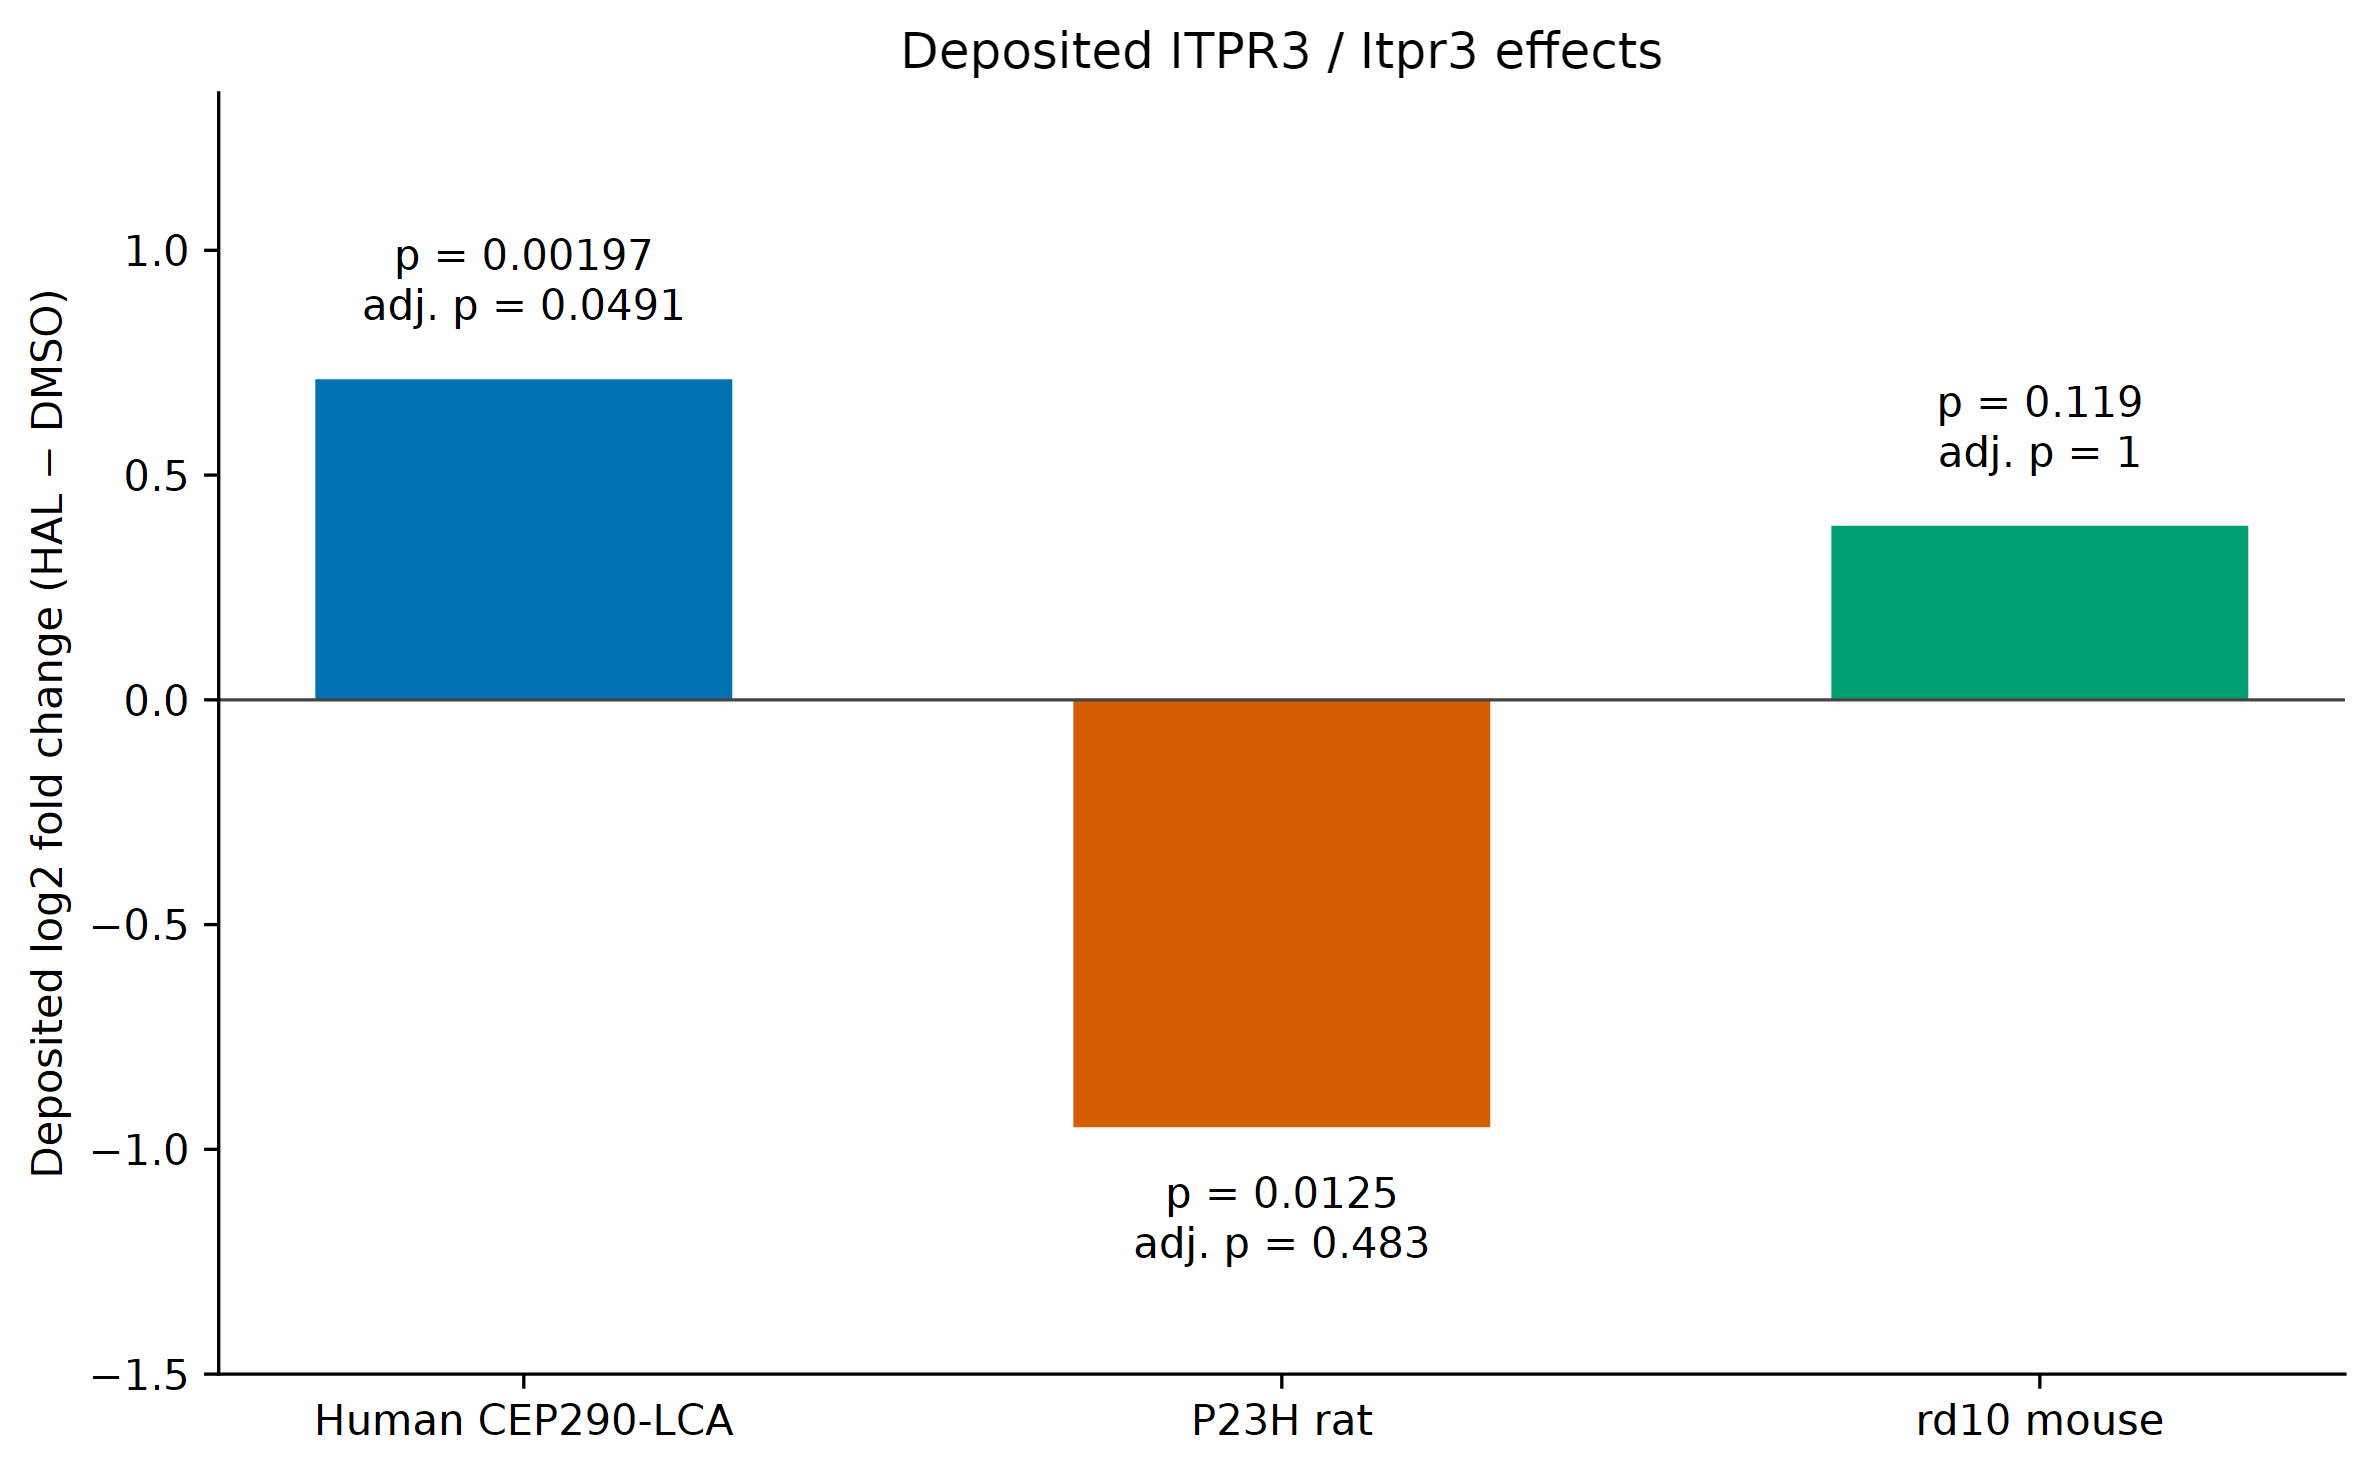
\includegraphics[width=\linewidth]{figures/figure1_deposited_itpr3.png}
\par\vspace{4pt}
{\small\raggedright \textbf{Figure 1. Deposited ITPR3/Itpr3 effects.} Bars show the deposited HAL-minus-DMSO log2 fold changes in human CEP290-LCA retinal organoids, P23H rat retina and rd10 mouse retina. Labels give the corresponding nominal and adjusted p-values, rounded for display. These are the source differential-expression table results, not recovered tests for Supplementary Figure S7B. Opposite effect directions or failure to cross a significance threshold do not establish absence of photoreceptor protection.\par}
\end{figure}
\subsection*{3.3 Expression matrices support the direction of the deposited effects}
The transformed-CPM contrasts closely tracked the deposited logFC columns. Human, P23H and rd10 Pearson correlations were 0.989, 0.962 and 0.916; Spearman correlations were 0.996, 0.975 and 0.963. Sign agreement was 98.6\%, 96.6\% and 94.6\%, respectively. This concordance supports the treatment-column interpretation and makes a simple reversal of treatment labels an unlikely explanation of the pairwise pattern. It does not validate every element of the original statistical model.

\subsection*{3.4 Replication obstacles and author communication}
Three unresolved details affect exact recovery: the S7A lists and mapping/selection code; the S7B sample-level values and test; and the PA/PB/PC/PD definitions and shared experimental units. Public labels separate all five patient HAL samples into PA/PB and all five DMSO samples into PC/PD. The codes may be bookkeeping labels, but that cannot be established from their names. We do not label them as proven batches or infer established confounding.

A request for these details was sent to the corresponding author on 27 September 2026.

\section*{4. Additional robustness analyses}
\subsection*{4.1 Threshold sensitivity and effect concordance}
{\small
\begin{longtable}{>{\raggedright\arraybackslash}p{\dimexpr 0.27\linewidth-2\tabcolsep\relax}>{\raggedright\arraybackslash}p{\dimexpr 0.15\linewidth-2\tabcolsep\relax}>{\raggedright\arraybackslash}p{\dimexpr 0.29\linewidth-2\tabcolsep\relax}>{\raggedright\arraybackslash}p{\dimexpr 0.29\linewidth-2\tabcolsep\relax}}
\toprule
\textbf{Model} & \textbf{Tested genes} & \textbf{Nominal p < 0.05 plus fold-change gate} & \textbf{Adjusted p < 0.05 plus fold-change gate} \\
\midrule
\endfirsthead
\toprule
\textbf{Model} & \textbf{Tested genes} & \textbf{Nominal p < 0.05 plus fold-change gate} & \textbf{Adjusted p < 0.05 plus fold-change gate} \\
\midrule
\endhead
\bottomrule\endfoot
Human CEP290-LCA & 12,265 & 3,640 & 513 \\
P23H rat & 12,037 & 876 & 0 \\
rd10 mouse & 11,702 & 235 & 0 \\
\end{longtable}
}
Under the adjusted-p gate, no gene qualifies in all three datasets because neither animal dataset has a qualifying gene. This is an evidence-threshold result, not an equivalence test or evidence that treatment has no molecular effect. Sample size, variation and model differences can all influence the numbers crossing a threshold.

\begin{figure}[htbp]
\centering
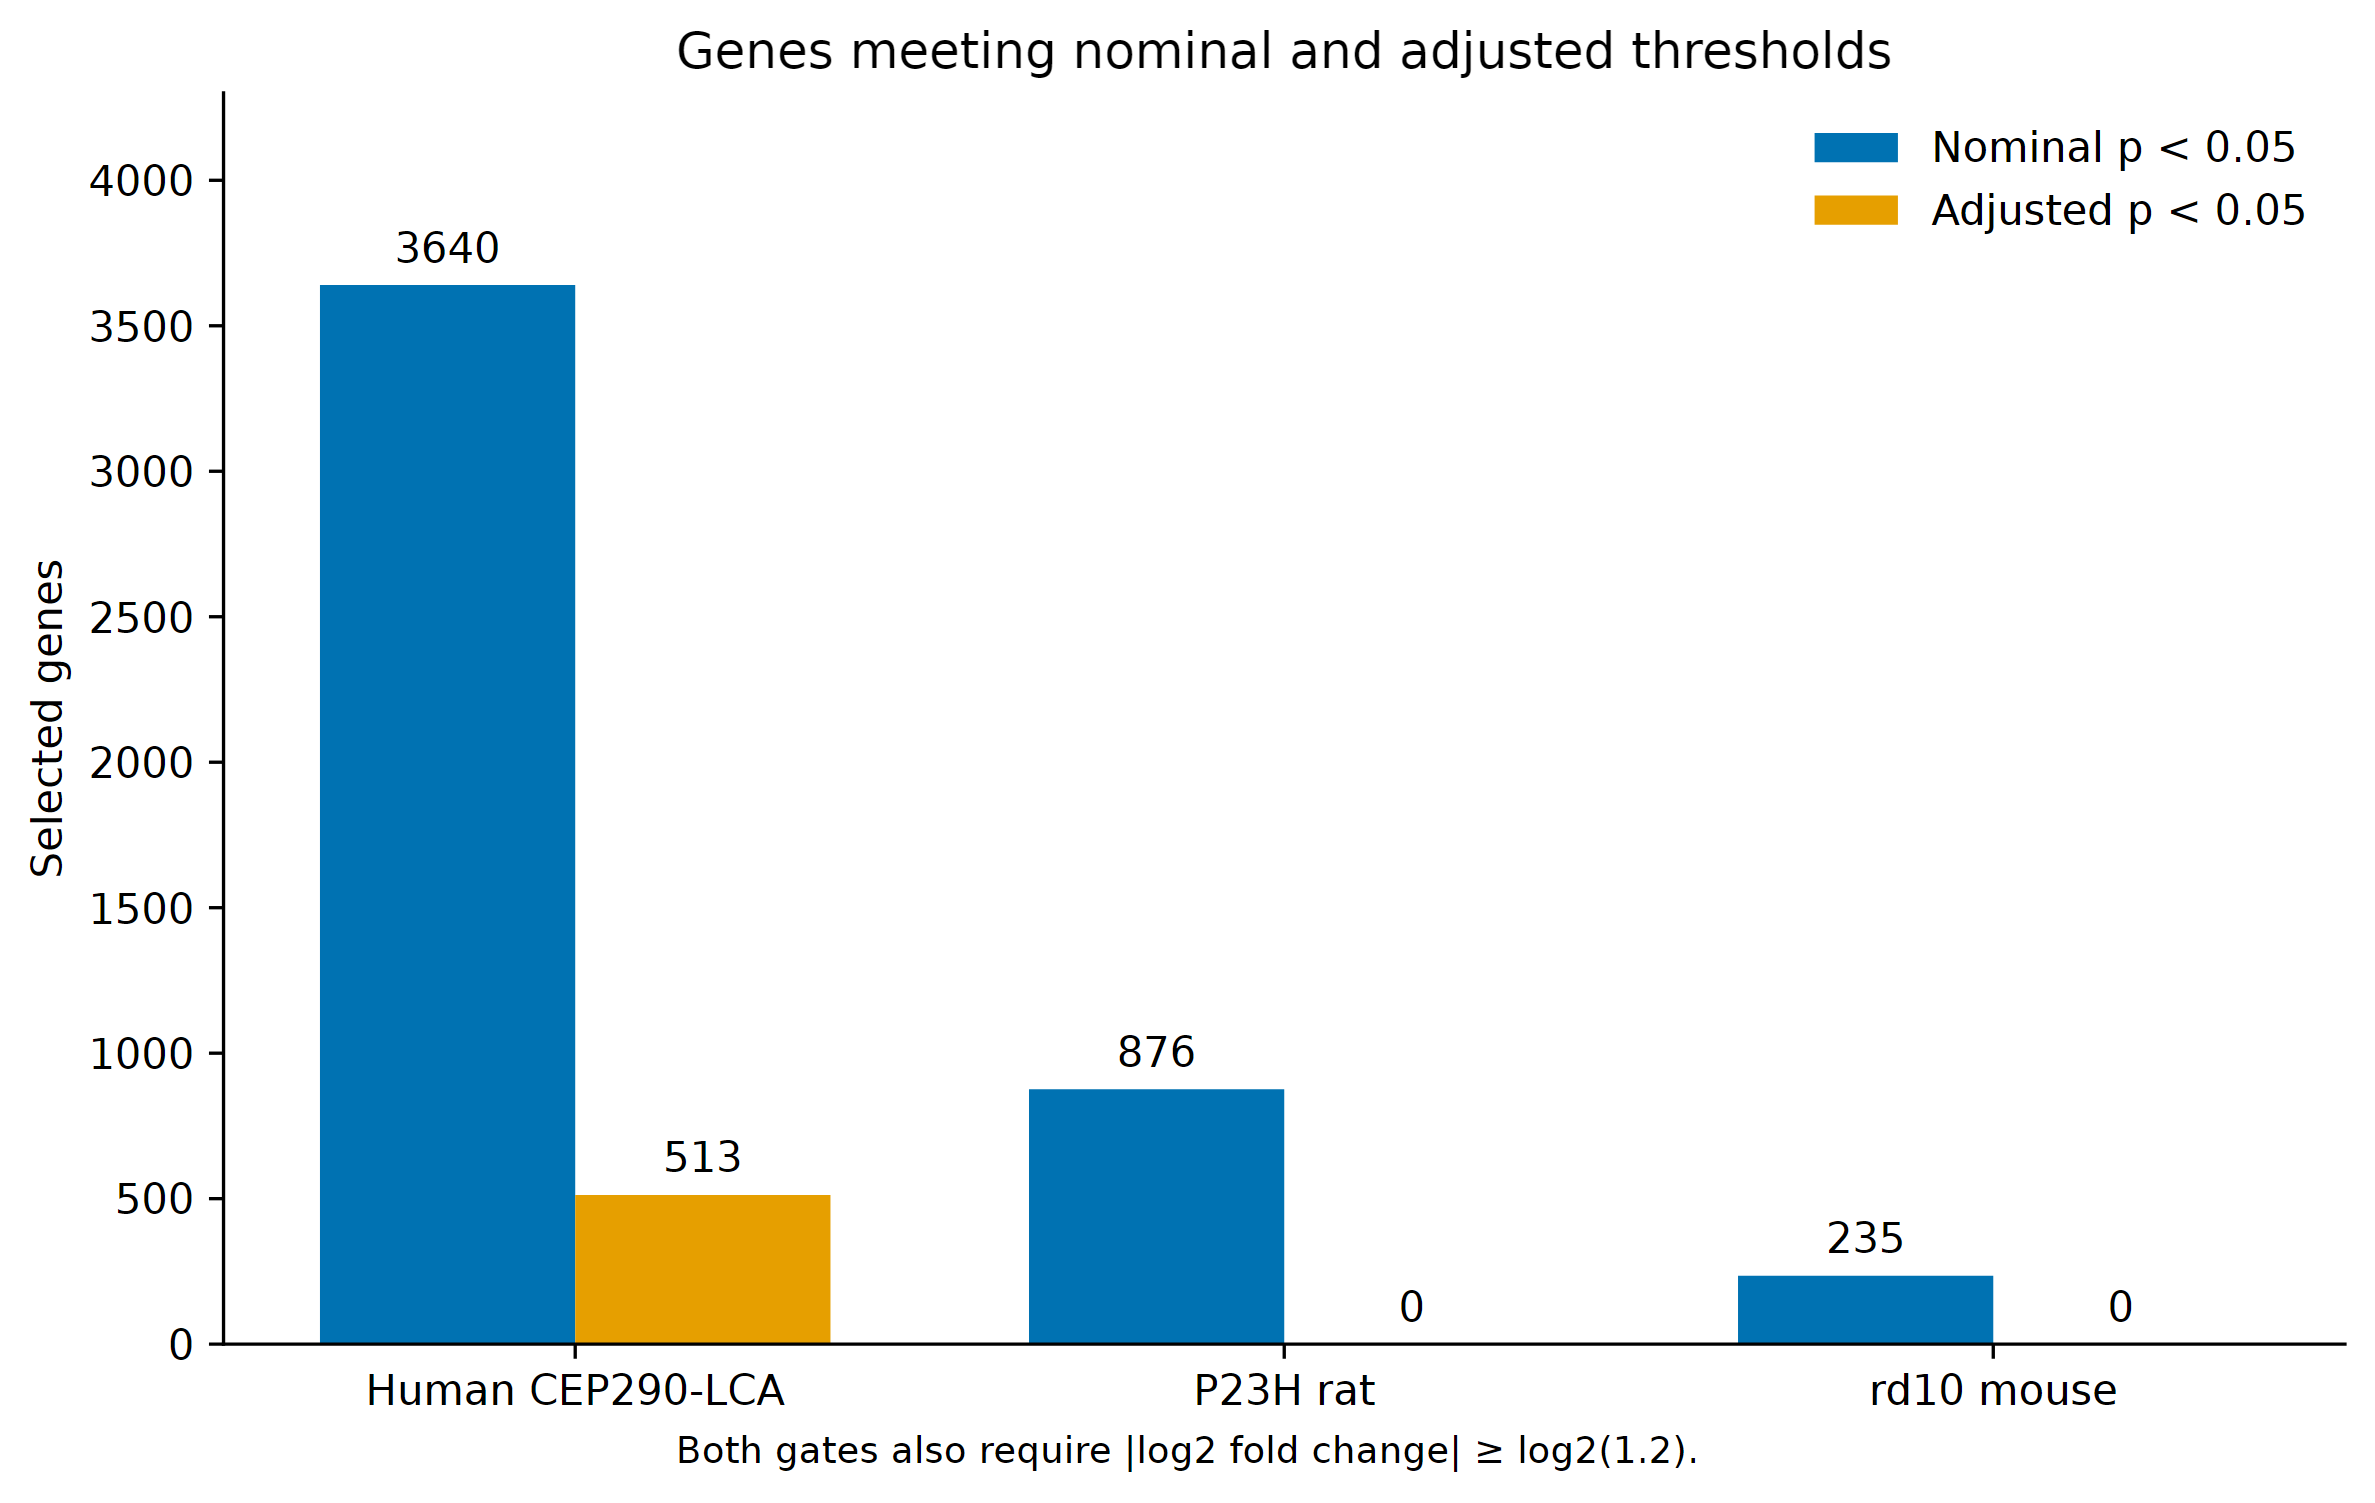
\includegraphics[width=\linewidth]{figures/figure2_gene_thresholds.png}
\par\vspace{4pt}
{\small\raggedright \textbf{Figure 2. Genes meeting nominal and adjusted thresholds.} Counts were obtained from the deposited differential-expression tables using nominal p < 0.05 or adjusted p < 0.05, with |log2 fold change| \ensuremath{\geq} log2(1.2) in both cases. Human, P23H and rd10 nominal counts were 3,640, 876 and 235; adjusted-threshold counts were 513, 0 and 0. These gates were applied to the source estimates without refitting the source model. Zero selected genes is not an equivalence test.\par}
\end{figure}
{\small
\begin{longtable}{>{\raggedright\arraybackslash}p{\dimexpr 0.21\linewidth-2\tabcolsep\relax}>{\raggedright\arraybackslash}p{\dimexpr 0.16\linewidth-2\tabcolsep\relax}>{\raggedright\arraybackslash}p{\dimexpr 0.15\linewidth-2\tabcolsep\relax}>{\raggedright\arraybackslash}p{\dimexpr 0.16\linewidth-2\tabcolsep\relax}>{\raggedright\arraybackslash}p{\dimexpr 0.16\linewidth-2\tabcolsep\relax}>{\raggedright\arraybackslash}p{\dimexpr 0.16\linewidth-2\tabcolsep\relax}}
\toprule
\textbf{Pair} & \textbf{One-to-one genes} & \textbf{Pearson r} & \textbf{Spearman rho} & \textbf{Cosine similarity} & \textbf{Sign agreement} \\
\midrule
\endfirsthead
\toprule
\textbf{Pair} & \textbf{One-to-one genes} & \textbf{Pearson r} & \textbf{Spearman rho} & \textbf{Cosine similarity} & \textbf{Sign agreement} \\
\midrule
\endhead
\bottomrule\endfoot
Human–P23H & 9,095 & \ensuremath{-}0.073 & \ensuremath{-}0.049 & \ensuremath{-}0.079 & 47.6\% \\
Human–rd10 & 8,943 & 0.247 & 0.306 & 0.250 & 62.4\% \\
P23H–rd10 & 9,364 & 0.073 & 0.081 & 0.062 & 52.4\% \\
\end{longtable}
}
The strongest pairwise concordance is human–rd10, while both comparisons involving P23H are weaker. These descriptive whole-vector statistics do not rule out a smaller shared gene set or a conserved response masked by cell composition, disease stage, dosing or measurement differences.

\subsection*{4.2 Sensitivity to sample removal}
Within-model median Spearman correlations between full and leave-one-out contrasts were 0.985, 0.966 and 0.912 for human, P23H and rd10, respectively. Their minima were 0.978, 0.797 and 0.679. Restricting genes to an absolute full-sample transformed-CPM contrast of at least log2(1.2), the minimum correlations were 0.957, 0.801 and 0.803.

Across full/deletion-state pairings, human–rd10 Spearman correlations remained positive (0.084–0.422; median 0.312). Human–P23H ranged from \ensuremath{-}0.244 to 0.198 (median \ensuremath{-}0.044), and P23H–rd10 from \ensuremath{-}0.139 to 0.284 (median 0.063). The positive human–rd10 association therefore persists across all tested deletion states, although individual deletions can substantially alter correlations involving P23H. Deleting one sample cannot resolve donor, batch or culture-level dependence.

\begin{figure}[htbp]
\centering
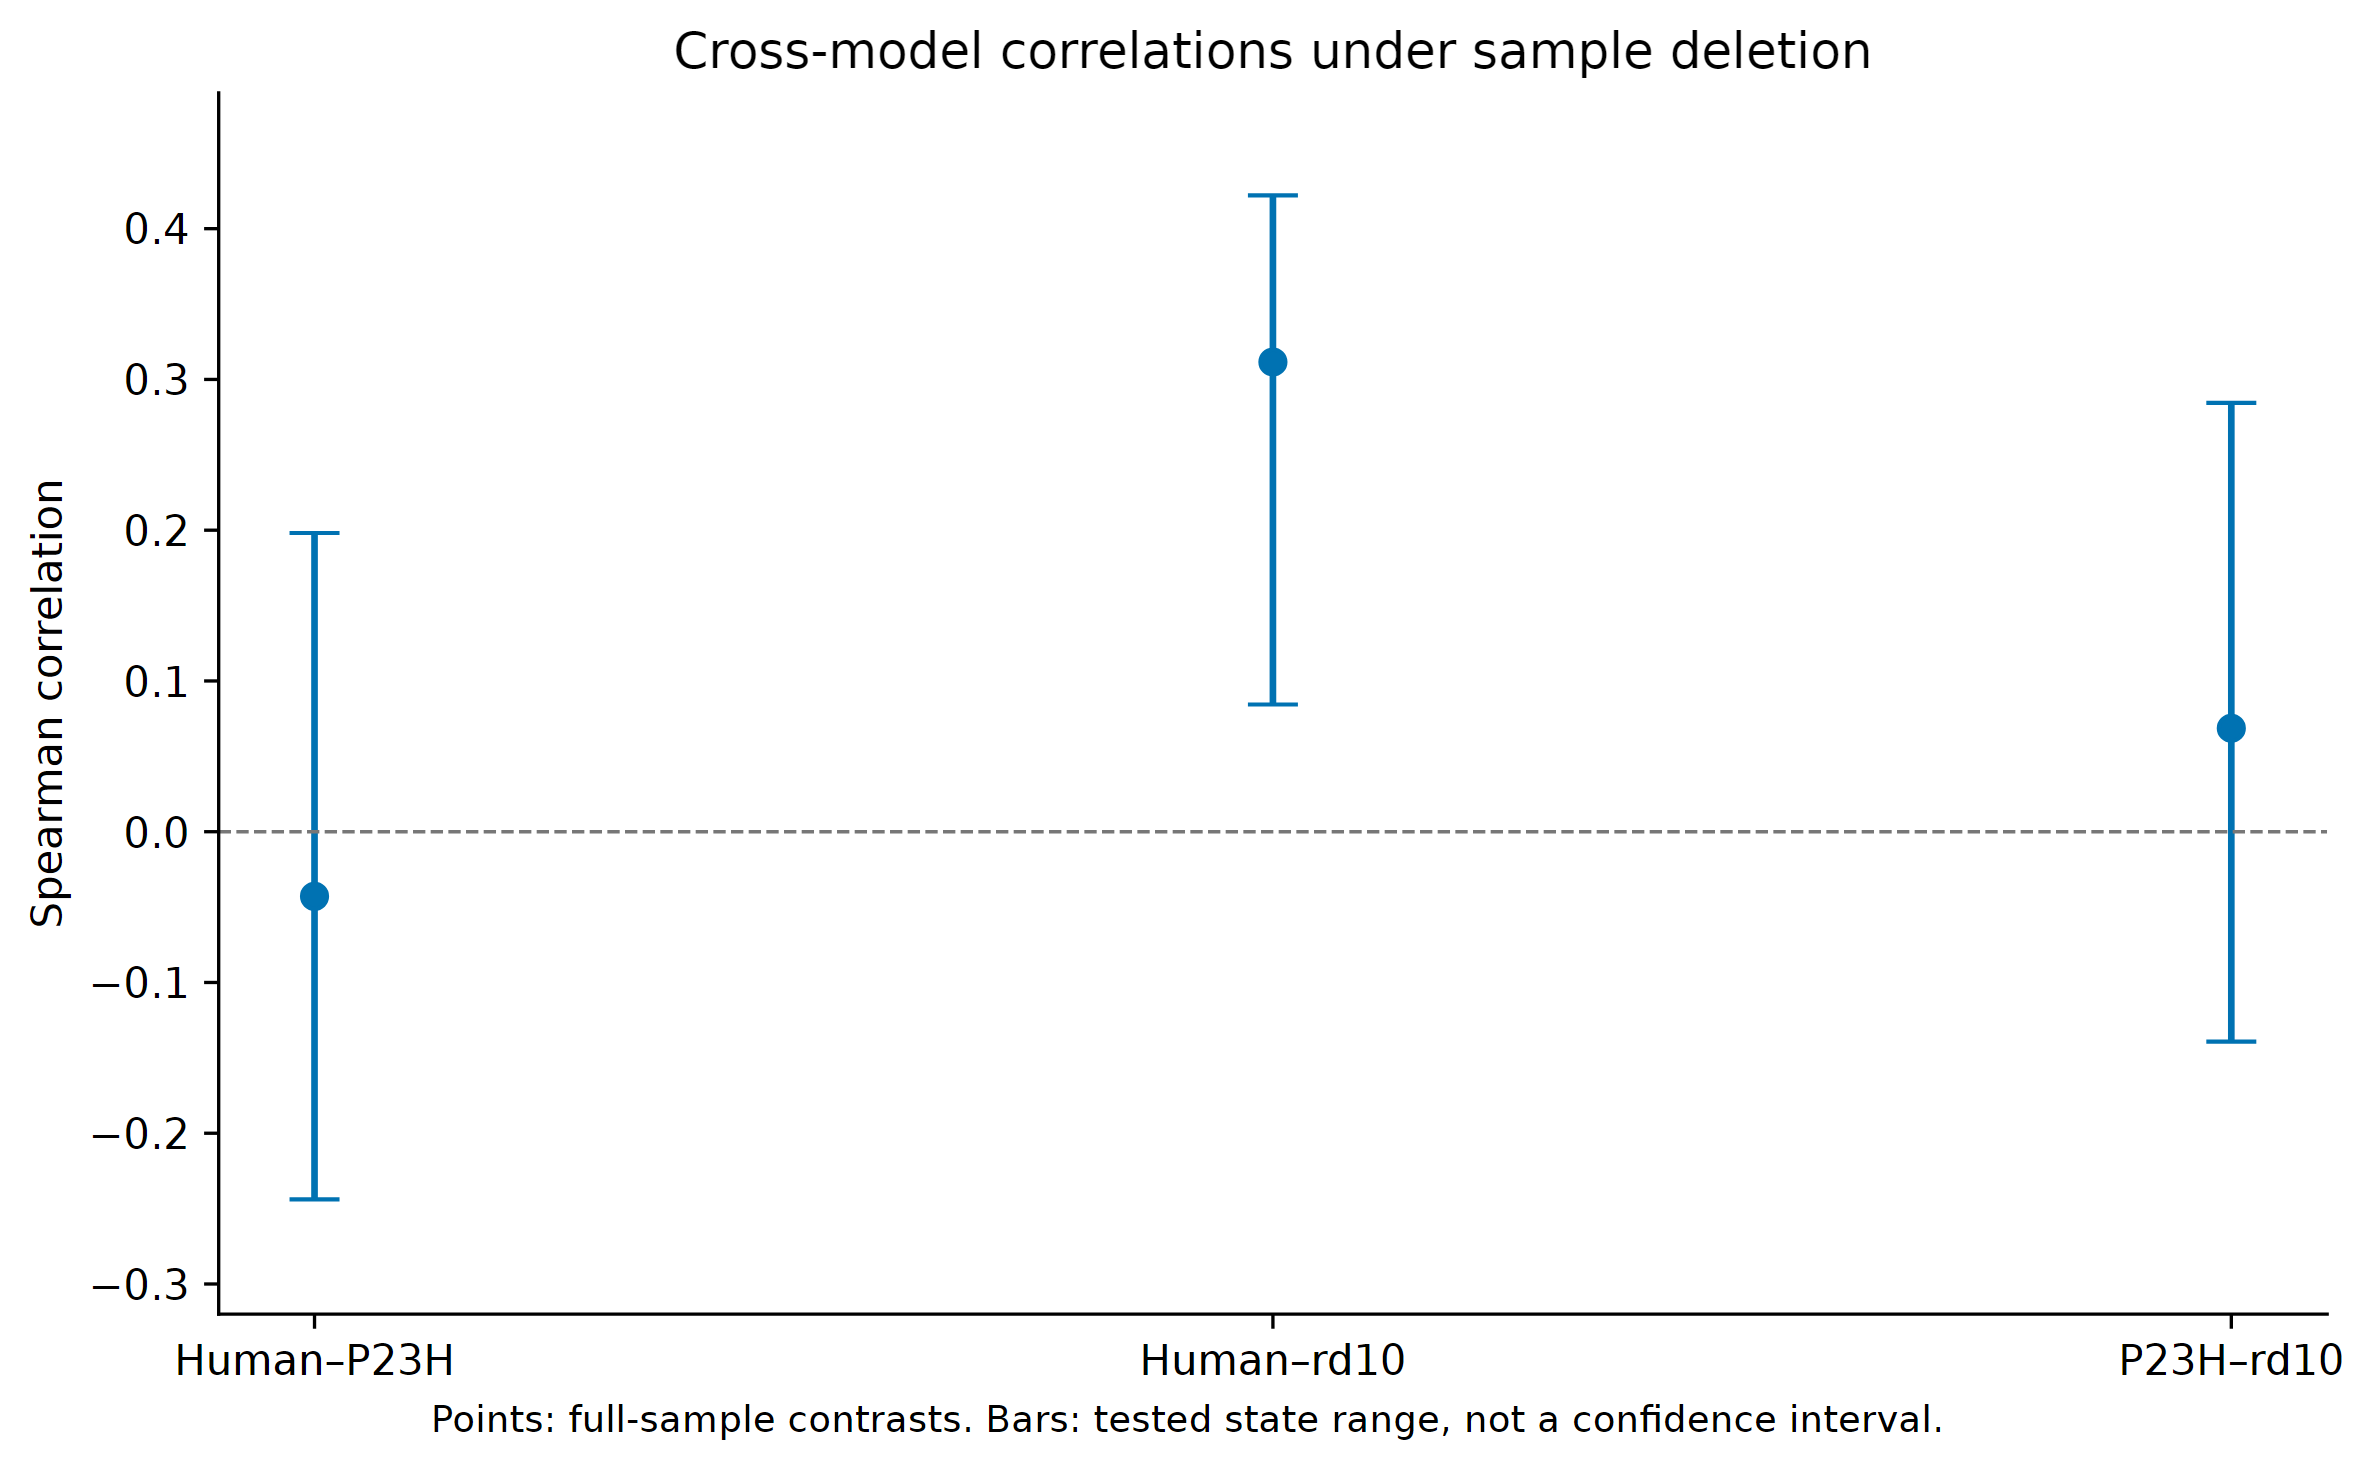
\includegraphics[width=\linewidth]{figures/figure3_deletion_ranges.png}
\par\vspace{4pt}
{\small\raggedright \textbf{Figure 3. Cross-model correlations under sample deletion.} Points show Spearman correlations between full-sample HAL-minus-DMSO mean contrasts of log2(CPM + 0.5), after one-to-one orthologue alignment. Bars span the minimum and maximum across all pairings of full and single-sample-deletion states: 110 human–P23H, 77 human–rd10 and 70 P23H–rd10 pairings. These sensitivity ranges are not confidence intervals. Human–rd10 remained positive in every tested state pairing; the two ranges involving P23H crossed zero.\par}
\end{figure}
The exhaustive label-assignment tail fractions for global separation were 0.0159, 0.198 and 0.300. These describe the selected statistic under the assumed exchangeability, not a causal test robust to unidentified experimental units.

\subsection*{4.3 A source-like overlap under a list-size-preserving null}
After one-to-one mapping and common-universe restriction, the source-like selected lists contained 663 human, 482 P23H and 160 rd10 genes. Fifty-five appeared in at least two lists, and one in all three. The random-set mean for at-least-two overlap was 56.9117 (standard deviation 6.8628), with Monte Carlo p = 0.62994. For the all-three intersection the mean was 0.6767 and p = 0.49475.

\begin{figure}[htbp]
\centering
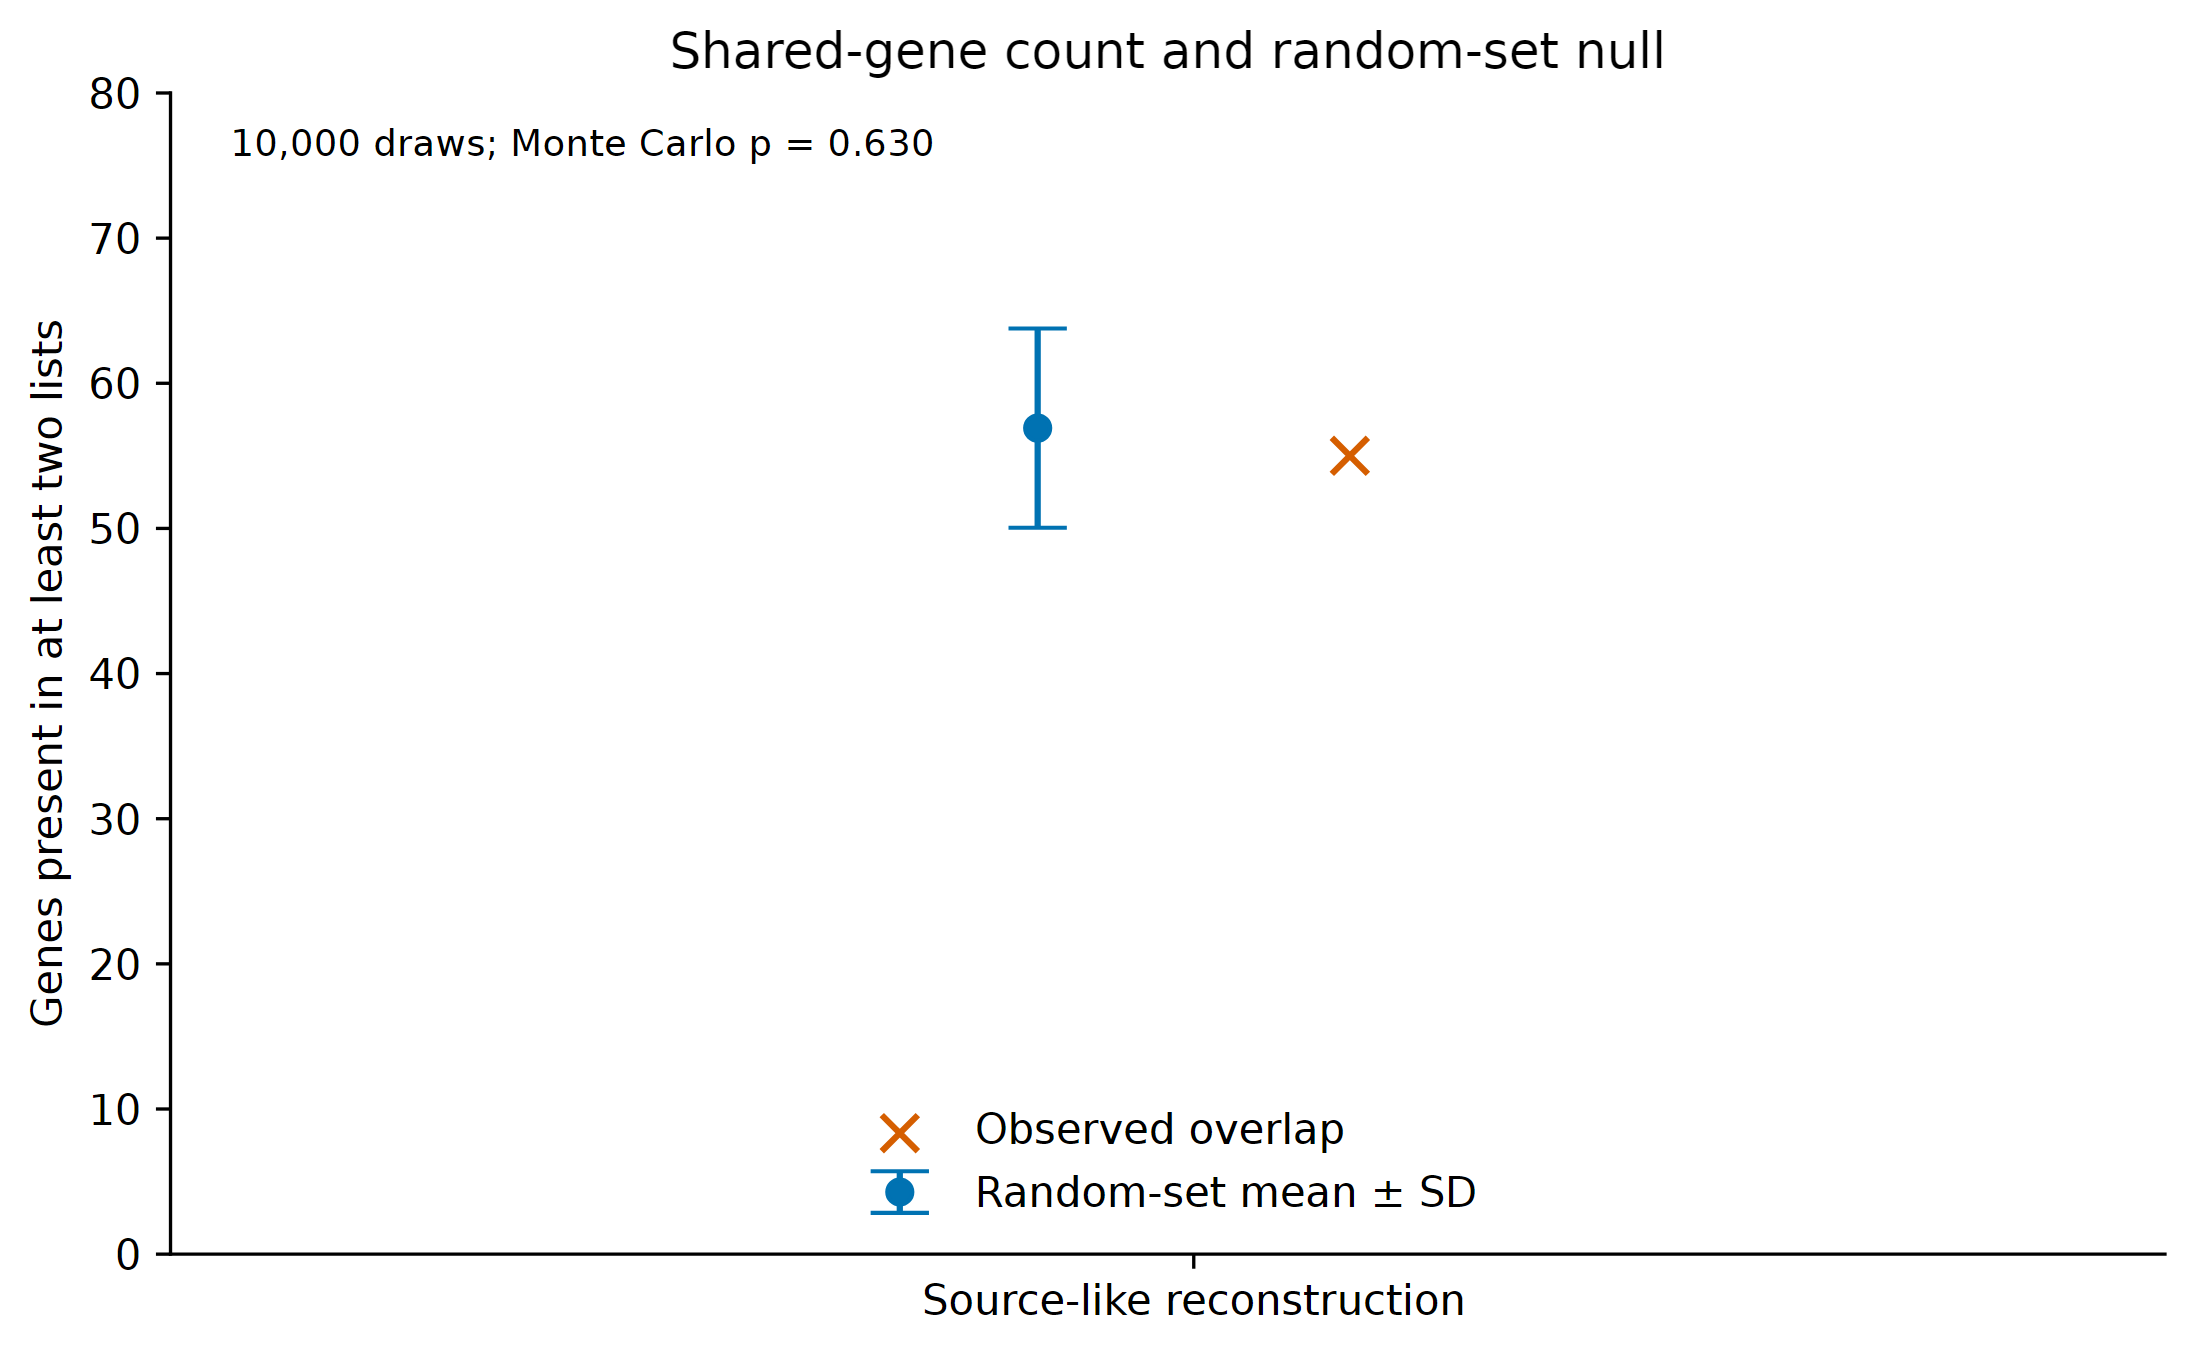
\includegraphics[width=\linewidth]{figures/figure4_overlap_null.png}
\par\vspace{4pt}
{\small\raggedright \textbf{Figure 4. Shared-gene count and random-set null.} The cross marks 55 genes shared by at least two source-like selected lists after one-to-one mapping and restriction to the common 8,645-gene universe. The point and bar show the mean and one standard deviation from 10,000 uniformly sampled sets preserving the three list sizes (663, 482 and 160). The upper-tail Monte Carlo probability, with the plus-one correction, was 0.630. The plot shows a summary, not the full null distribution. These are not the recovered S7A lists, and the null does not preserve gene co-expression or gene-specific detectability.\par}
\end{figure}
Those overlap counts are not unusual under this particular null. The calculation does not assign a p-value to the source's 46 shared genes, because our selected lists are not the recovered S7A lists. Uniform random sets also make no allowance for biological correlation among genes. The useful result is conditional: overlap size alone does not establish an enrichment beyond what these list sizes would produce.

\subsection*{4.4 Pathway direction and threshold crossing differ}
Ranked GSEA returned 3, 154 and 2 pathways at FDR < 0.05 for human, P23H and rd10, with none crossing that threshold in all three. For oxidative phosphorylation, normalized enrichment scores were +1.513, +3.532 and +1.729, with returned FDR estimates 0.196, 0 and 0.432. Its positive direction is shared; the selected significance threshold is crossed only in P23H.

Ribosome had scores +2.342, +3.202 and +0.938, with FDR estimates 0.00057, 0 and 1.0. Circadian entrainment did not meet FDR < 0.05 in any model and had a negative score in P23H but positive scores in the other two. These results retain shared directional evidence in some pathways while quantifying how strongly it depends on the analysis and threshold. They neither refute the source's partial-similarity interpretation nor establish a common causal mechanism.

\begin{figure}[htbp]
\centering
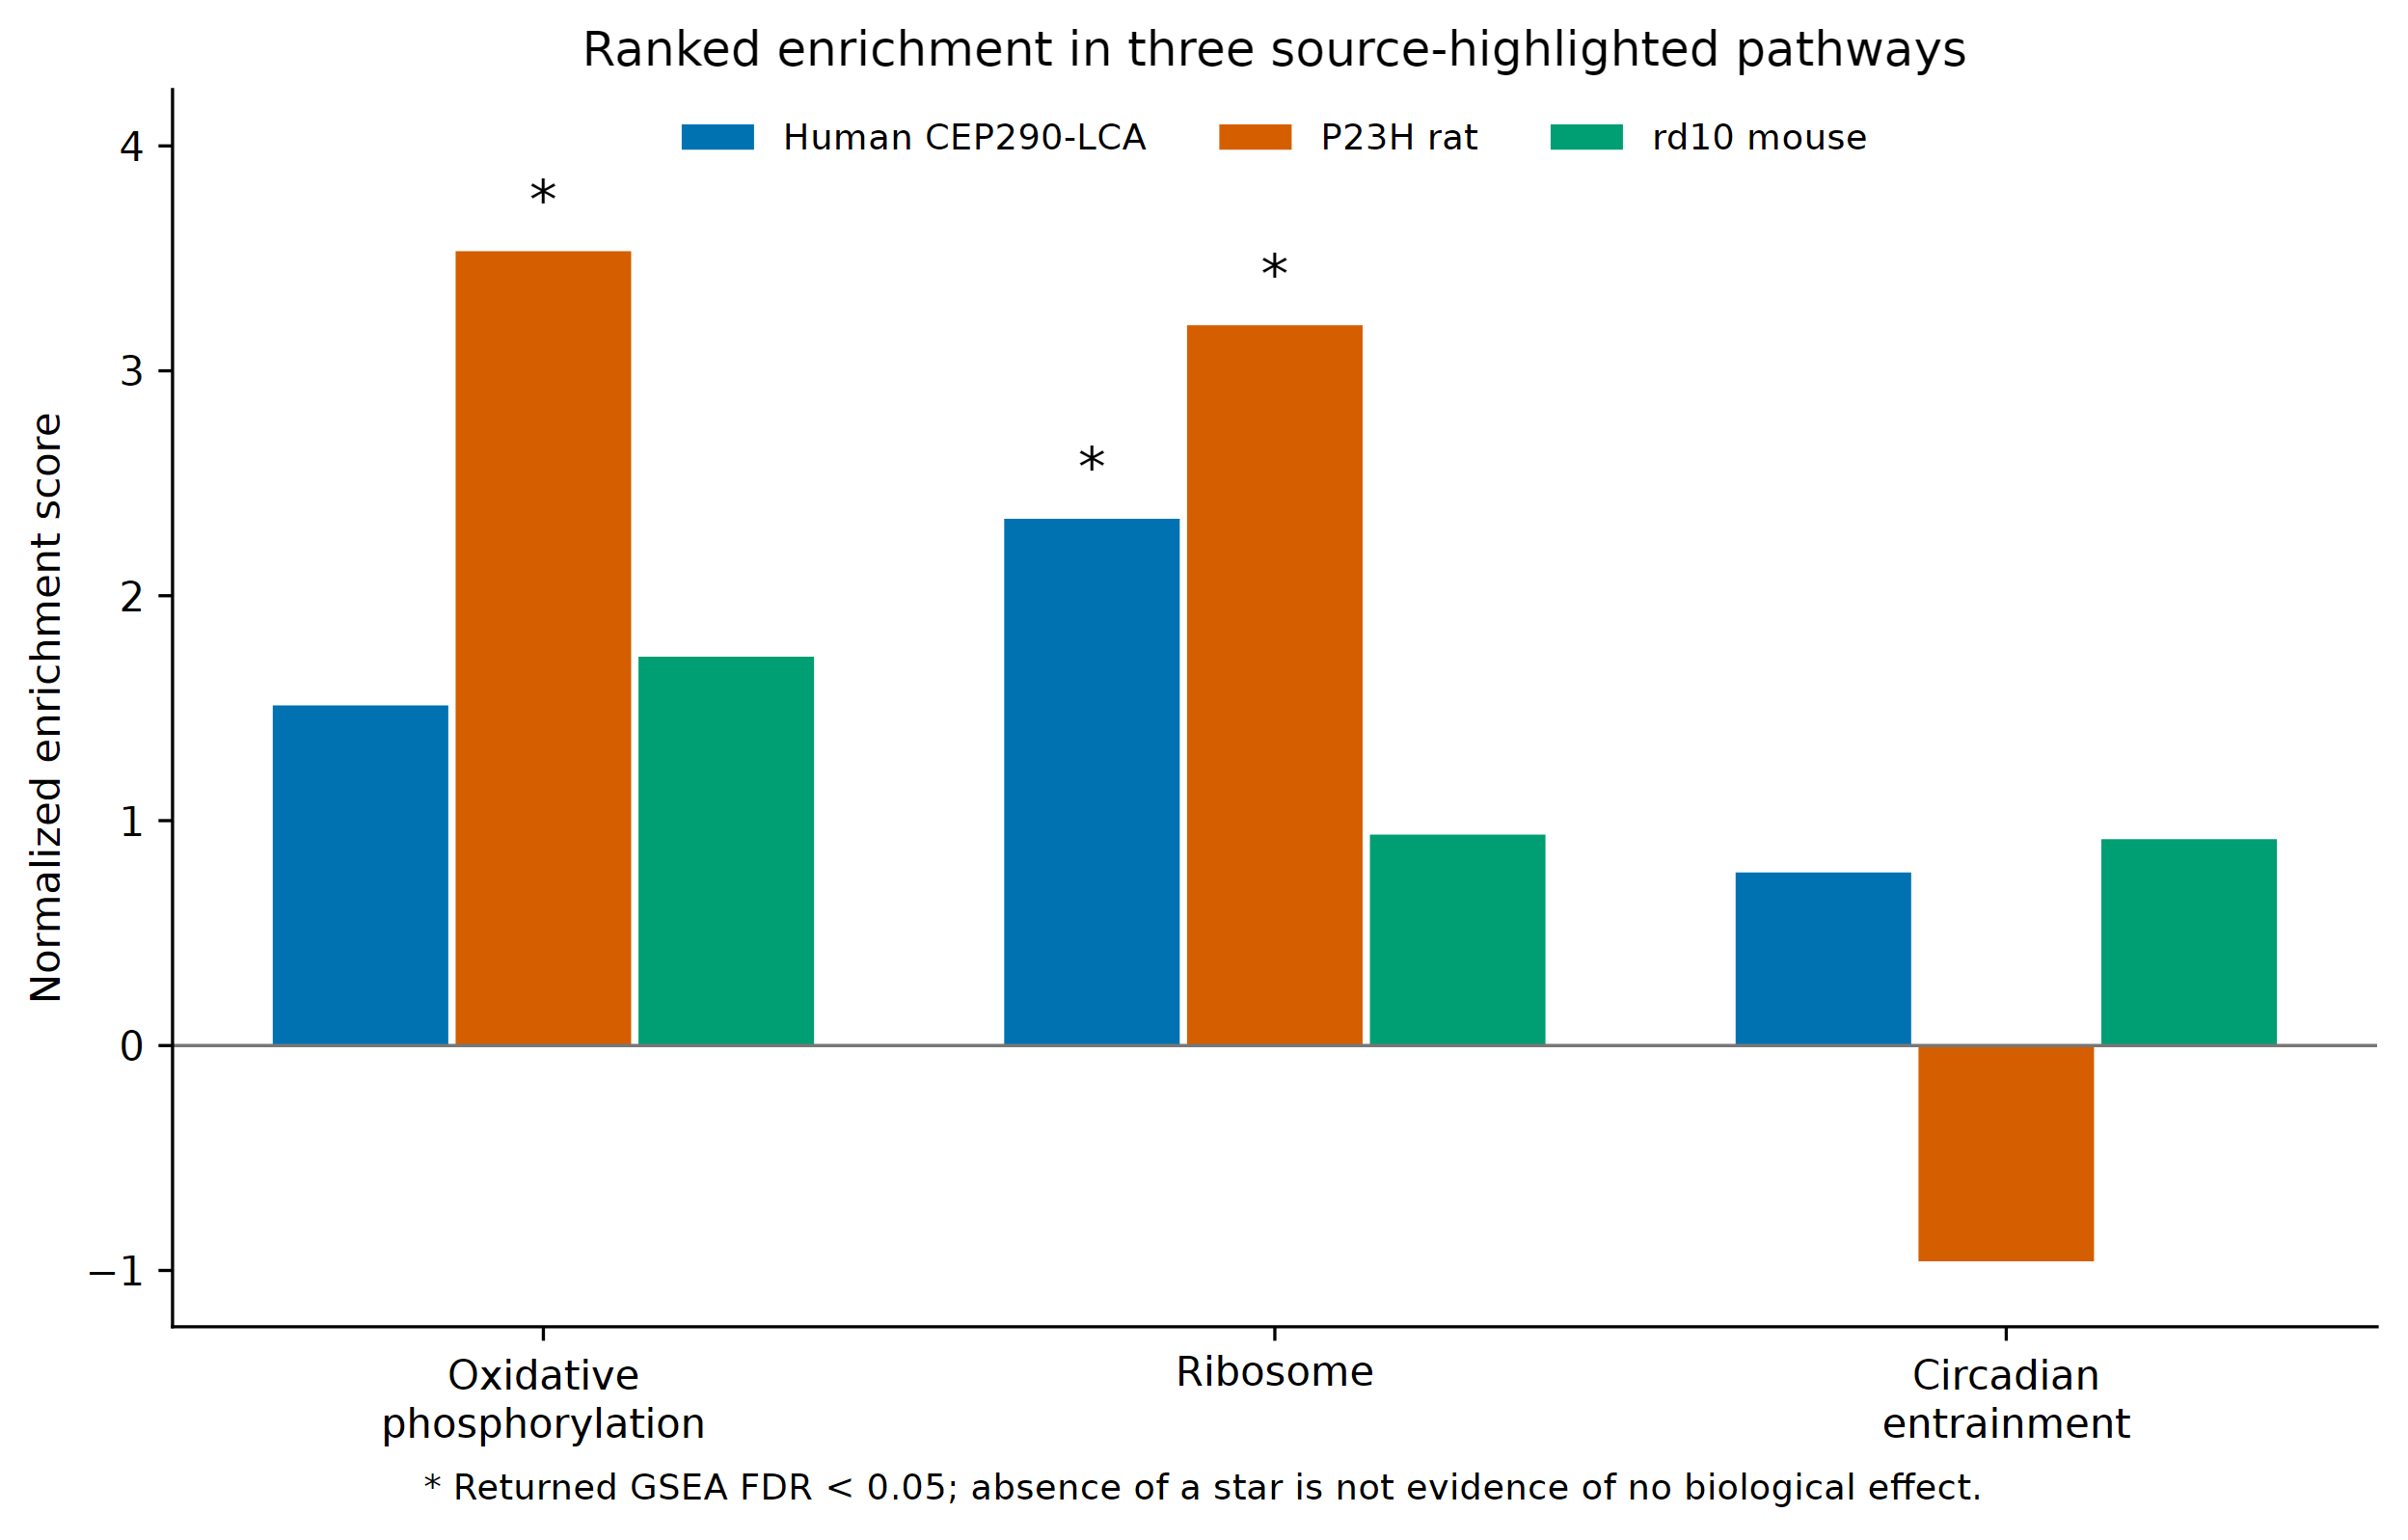
\includegraphics[width=\linewidth]{figures/figure5_ranked_pathways.png}
\par\vspace{4pt}
{\small\raggedright \textbf{Figure 5. Ranked enrichment in three source-highlighted pathways.} Bars show normalized enrichment scores for oxidative phosphorylation, ribosome and circadian entrainment, calculated with GSEApy prerank from deposited moderated t-statistics. The analysis used 8,644 common one-to-one symbols, KEGG\_2021\_Human sets with 10–500 represented genes, 2,000 permutations and seed 20260921; 277 pathways were tested per model. Stars denote returned FDR estimates below 0.05. A returned zero estimate is not a literal probability of zero. The dated 27 September library snapshot reproduced the checked archived values but is not established as byte-identical to the historical input. This ranked analysis differs from the source's selected-gene pathway procedure.\par}
\end{figure}
\section*{5. Execution record and reproducibility limits}
The 27 September replay executed the full core analysis, overlap randomization, ranked GSEA, all 25 sample deletions and all label assignments. It matched 26 archived central quantities, 27 rounded leave-one-out/permutation quantities and 18 displayed pathway quantities. These checks cover the reported comparisons; they are not a claim that every historical output file was recovered byte-for-byte. Core runs under Python hash seeds 1 and 77 produced identical result files. The preserved code already sorts the sampling universe; no scientific determinism repair was needed.

The current environment used Python 3.12.10, NumPy 2.5.3, pandas 2.3.3, SciPy 1.18.1, requests 2.34.2 and GSEApy 1.3.1. The historical logs listed pandas 3.0.6, so runtime identity is not claimed. Adapters redirected data requests to preserved files and supplied local mapping and pathway inputs without changing the scientific arithmetic. Analysis runs made no outbound network requests.

The full pipeline was also executed from a new isolated environment in an empty workspace. Both core runs and the ranked-pathway and leave-one-out results were byte-identical to the preserved reanalysis outputs; six bounded reconstruction files likewise matched. All five figures were generated from these new outputs, not copied from earlier runs. These checks establish reproducibility of the specified reanalysis, not recovery of the source authors' unpublished choices.

The KEGG\_2021\_Human library was downloaded from the official Enrichr endpoint on 27 September 2026. It contained 320 terms before analysis filters; its raw SHA-256 is \nolinkurl{566763b3402ee1f06612cc48b57e2a0f3f92a9a9e7d1871cc2da9f940e2d609a}. No raw library file or hash was retained for the historical run. Matching the checked results does not prove that the newly preserved library is byte-identical to the one previously used. This dated input must remain distinguishable from the historical result archive.

All pre-existing local inputs, scripts and manuscript versions were preserved unchanged. The current analysis starts from processed expression data and cannot rule out errors introduced before deposition. It also cannot supply the missing source-figure specification or establish independence of biological replicates from unresolved sample names.

\section*{6. Discussion}
The most consequential gap is concrete: the deposited rd10 Itpr3 test and the source's all-three significance statement are not yet connected by a recoverable figure-level test. Likewise, the available S7A description admits choices whose outputs differ, and none of our nine candidates reproduces its full intersection structure. Sharing the figure-source tables and generating code could settle these questions without new animal or organoid experiments.

The additional analyses answer a different question: what remains stable under explicitly stated changes to the treatment-effect comparison? Human–rd10 concordance survives every tested single-sample deletion, and oxidative-phosphorylation enrichment retains a positive direction across models. At the same time, gene-level threshold crossing, pairwise correlations and pathway FDR values differ substantially. These observations give numerical detail to partial molecular similarity rather than overturning it.

A common therapeutic outcome does not require every responsive model to have an identical transcriptome. Our results do not decide whether halofantrine protects photoreceptors, which target mediates protection, or whether the drug is safe for clinical use. They provide a reproducible account of the deposited transcriptomic evidence, identify which figure-level results remain unresolved, and keep the robustness extensions separate from exact source replication.

\section*{Appendix A. Region counts for the nine S7A reconstruction rules}
Rule labels refer to the selection procedures in Section 3.1. Pairwise columns exclude the third model. H denotes human CEP290-LCA, R P23H rat and M rd10 mouse. Counts use the all-homologue mapping described in Section 2.2, not the one-to-one mapping used for robustness extensions.

{\small
\begin{longtable}{>{\raggedright\arraybackslash}p{\dimexpr 0.16\linewidth-2\tabcolsep\relax}>{\raggedright\arraybackslash}p{\dimexpr 0.12\linewidth-2\tabcolsep\relax}>{\raggedright\arraybackslash}p{\dimexpr 0.12\linewidth-2\tabcolsep\relax}>{\raggedright\arraybackslash}p{\dimexpr 0.12\linewidth-2\tabcolsep\relax}>{\raggedright\arraybackslash}p{\dimexpr 0.12\linewidth-2\tabcolsep\relax}>{\raggedright\arraybackslash}p{\dimexpr 0.12\linewidth-2\tabcolsep\relax}>{\raggedright\arraybackslash}p{\dimexpr 0.12\linewidth-2\tabcolsep\relax}>{\raggedright\arraybackslash}p{\dimexpr 0.12\linewidth-2\tabcolsep\relax}}
\toprule
\textbf{Rule} & \textbf{H only} & \textbf{R only} & \textbf{M only} & \textbf{H–R only} & \textbf{H–M only} & \textbf{R–M only} & \textbf{All three} \\
\midrule
\endfirsthead
\toprule
\textbf{Rule} & \textbf{H only} & \textbf{R only} & \textbf{M only} & \textbf{H–R only} & \textbf{H–M only} & \textbf{R–M only} & \textbf{All three} \\
\midrule
\endhead
\bottomrule\endfoot
Source S7A & 470 & 379 & 405 & 16 & 13 & 16 & 1 \\
R1 & 450 & 376 & 329 & 18 & 24 & 36 & 8 \\
R2 & 466 & 427 & 448 & 22 & 12 & 15 & 0 \\
R3 & 466 & 427 & 448 & 22 & 12 & 15 & 0 \\
R4 & 450 & 376 & 329 & 18 & 24 & 36 & 8 \\
R5 & 464 & 409 & 377 & 21 & 15 & 16 & 0 \\
R6 & 466 & 414 & 189 & 21 & 13 & 11 & 0 \\
R7 & 450 & 373 & 312 & 16 & 25 & 41 & 9 \\
R8 & 469 & 421 & 360 & 21 & 10 & 9 & 0 \\
R9 & 470 & 424 & 198 & 21 & 9 & 6 & 0 \\
\end{longtable}
}
\section*{Data and code availability}
The source expression data are available under GSE327435 and its three named subseries. The reanalysis preserves compressed-input hashes, selection rules, mapping provenance, execution environment and result-comparison records.

\section*{Author information and declarations}
Byungwoong Yoo directed the research question and reanalysis workflow. No new human-participant or animal experiments were undertaken.

\textbf{Funding.} This work received no external funding.

\textbf{Competing interests.} In September 2026, the author made preliminary inquiries to the US National Institutes of Health about potential licensing and the patent status of halofantrine-related retinal technology.

\textbf{AI assistance.} OpenAI Codex assisted with analysis scripts, reproducibility checks, and manuscript drafting and editing.

\section*{References}
1. Kim M, et al. Halofantrine protects photoreceptors in multiple models of retinal degeneration. Research Square, version 1, 13 May 2026. \url{https://doi.org/10.21203/rs.3.rs-9511432/v1}

2. Barrett T, et al. NCBI GEO: archive for functional genomics data sets—update. Nucleic Acids Research. 2013;41:D991–D995. \url{https://doi.org/10.1093/nar/gks1193}

3. Song HB, et al. Sex-specific attenuation of photoreceptor degeneration by reserpine in a rhodopsin P23H rat model of autosomal dominant retinitis pigmentosa. eLife. 2025;14:RP103888. \url{https://doi.org/10.7554/eLife.103888}

4. Yates AD, et al. Ensembl 2026. Nucleic Acids Research. 2026;54:D1053–D1060. \url{https://doi.org/10.1093/nar/gkaf1239}

5. Fang Z, Liu X, Peltz G. GSEApy: a comprehensive package for performing gene set enrichment analysis in Python. Bioinformatics. 2023;39:btac757. \url{https://doi.org/10.1093/bioinformatics/btac757}

6. Kanehisa M, Furumichi M, Sato Y, Kawashima M, Ishiguro-Watanabe M. KEGG for taxonomy-based analysis of pathways and genomes. Nucleic Acids Research. 2023;51:D587–D592. \url{https://doi.org/10.1093/nar/gkac963}

7. Xie Z, et al. Gene set knowledge discovery with Enrichr. Current Protocols. 2021;1:e90. \url{https://doi.org/10.1002/cpz1.90}

\end{document}
